\taskpic{Из среды с показателем преломления $n_0$ в неоднородную среду 
с показателем преломления $n = n_0 \sqrt{1-\frac yH}$ под углом $\varphi_0$ входит 
луч света. На какую максимальную глубину сможет проникнуть луч? 
При каком значении угла падения $\varphi_0$ расстояние между точками 
входа и выхода луча максимально?}{
\begin{tikzpicture}[>=latex]
  \fill[gray!10] (0.2,2) rectangle ++(3.6,-2);
  \draw[thick] (0.2,2) -- ++(3.6,0);
  \draw[dashed,thick,->] (2,3.5) -- ++(0,-3) node [right] {$y$};
  \draw[very
  thick,draw=red,postaction=decorate,decoration={markings,mark=at
    position .55 with {\arrow[red]{>}}}] (1,3.5) -- (2,2);
  \draw[blue] (2,2.5) arc (90:90+atan(2/3):0.5);
  \draw[blue] (1.8,2.7) node {$\alpha$};
  \draw (0.5,3) node {$n_0$};
  \draw (0.7,1) node {$n(y)$};
\end{tikzpicture}
}

\task{На какую минимальную высоту надо поднять поршень, лежащий на 
поверхности воды в герметичном сосуде, чтобы вся вода в нем 
испарилась? Толщина слоя воды от дна сосуда --- $h$, плотность воды 
--- $\rho$, молярная масса --- $\mu$, давление насыщенного водяного пара 
$p$. Температура $T$ воды и пара в сосуде поддерживается постоянной.}

\task{Тонкая доска массой $m_1$ и длиной $L$ скользит по гладкому столу 
со скоростью $v_1$. Маленькая шайба массой $m_2$ плавно въезжает на 
доску со скоростью $v_2$ относительно Земли. При каких значениях 
коэффициента трения между доской и шайбой потери механической 
энергии при их взаимодействии максимальны?}

\task{Груз поднимают при помощи невесомого поршня, скользящего без 
трения в вертикальном теплоизолированном цилиндре. Под поршнем 
находится идеальный одноатомный газ, медленно нагреваемый при 
помощи электронагревателя с КПД, равным $\eta = 1/2$. Определить КПД 
подъемного устройства, если атмосферное давление отсутствует.}

\taskpic{В точках A и B жесткого невесомого стержня укреплены два 
маленьких шарика. В точке O стержень закреплен и может свободно 
вращаться в вертикальной плоскости. В начальный момент времени 
стержень отклоняют от вертикального положения на очень 
маленький угол и отпускают. Найти силу, действующую на шарик В со 
стороны стержня в момент, когда угол между стержнем и вертикалью 
равен $\alpha$. Масса каждого груза $m$, длина стержня $L$, 
OA=AB.}{
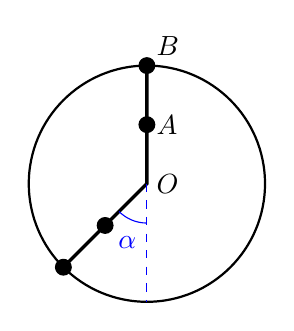
\begin{tikzpicture}[>=latex]
  \draw[thick] (2,2) circle (1.5);
  \draw[very thick] (2,3.5) -- (2,2) -- ++(-135:1.5);
  \filldraw[black] (2,2.75) circle (0.1) node[right] {$A$};
  \filldraw[black] (2,3.5) circle (0.1) node[above right] {$B$};
  \draw (2,2) node[right] {$O$};
  \filldraw[black] (2,2) ++(-135:0.75) circle (0.1);
  \filldraw[black] (2,2) ++(-135:1.5) circle (0.1);

  \draw[dashed,blue] (2,2) -- ++(0,-1.5);
  \draw[blue] (2,2) ++ (0,-0.5) arc (-90:-135:0.5);
  \draw[blue] (1.75,1.25) node {$\alpha$};
\end{tikzpicture}
}

\task{Протон (ядро атома водорода) и альфа-частица (ядро атома гелия, 
состоящее из двух протонов и двух нейтронов) разгоняются 
одинаковой ускоряющей разностью потенциалов и влетают в 
однородное магнитное поле перпендикулярно его линиям. 
Определить отношение радиусов орбит и нарисовать траектории 
движения частиц в магнитном поле. Массы протона и нейтрона равны.}

\taskpic{Верхняя поверхность большой плоской пластины 
поддерживается при постоянной температуре $T_1$, а нижняя --- при 
температуре $T_2$ ($T_2>T_1$). Оцените подъемную силу 1~м$^2$ такой 
пластины, если она находится в атмосфере разреженного газа с 
давлением $p_0$ и температурой $T_0$ ($T_1<T_0<T_2$).}{
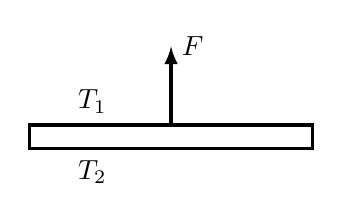
\begin{tikzpicture}[>=latex]
  \draw[very thick] (0.2,2) rectangle ++(3.6,-0.3);
  \draw (1,2.3) node {$T_1$};
  \draw (1,1.4) node {$T_2$};
  \draw[very thick,->] (2,2) -- ++(0,1) node[right] {$F$};
\end{tikzpicture}
}

\task{На одном из островов Бермудского треугольника ускорение 
свободного падения отклонено на юг и составляет угол $\alpha$ с 
вертикалью. На каком расстоянии от туземца упадет стрела, 
выпущенная им вертикально вверх с начальной скоростью $v_0$? В 
каком направлении следует выпустить стрелу для того, чтобы она 
вернулась обратно?}

\taskpic{Равнобедренный треугольник состоит из 3 маленьких шариков, 
скрепленных невесомыми жесткими стержнями. Заряд верхнего 
шарика $2\alpha q$, а заряды каждого из нижних шариков равны $(1-\alpha)q$. 
Массы шариков одинаковы. Эта конструкция находится в равновесии 
в сонаправленных гравитационном поле $g$ и электростатическом 
поле $E$. Определить устойчивость равновесия в зависимости от 
параметра $\alpha$.}{
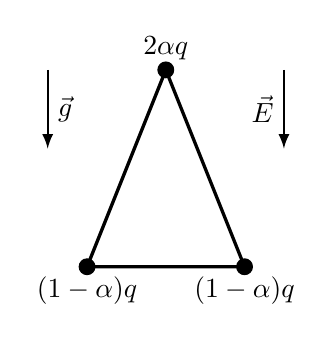
\begin{tikzpicture}[>=latex]
  \coordinate (a) at (1,1);
  \coordinate (b) at (2,3.5);
  \coordinate (c) at (3,1);
  \draw[very thick] (a) -- (b) -- (c) -- cycle;
  \filldraw[black] (a) circle (0.1) node [below] {$(1-\alpha) q$};
  \filldraw[black] (b) circle (0.1) node [above] {$2\alpha q$};
  \filldraw[black] (c) circle (0.1) node [below] {$(1-\alpha) q$};
  \draw[thick,->] (0.5,3.5) -- ++(0,-1) node[midway,right] {$\vec{g}$};
  \draw[thick,->] (3.5,3.5) -- ++(0,-1) node[midway,left] {$\vec{E}$};
\end{tikzpicture}
}

\taskpic{Две частицы, имеющие заряды $q_1$ и $q_2$ и равные массы, могут 
скользить без трения вдоль двух параллельных прямых, 
расположенных на расстоянии $L$. В начальный момент частица $q_1$ 
движется со скоростью $v_0$ из бесконечности, приближаясь к 
покоящейся частице $q_2$. Определить установившиеся скорости 
частиц.}{
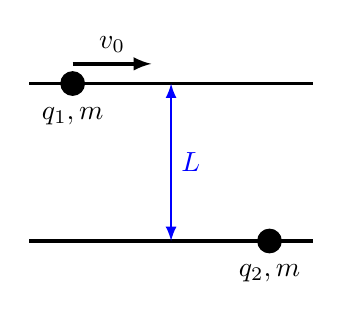
\begin{tikzpicture}[>=latex]
  \draw[very thick] (0.2,3) -- +(3.6,0);
  \draw[very thick] (0.2,1) -- +(3.6,0);
  \draw[thick,blue,<->] (2,3) -- +(0,-2) node[midway,right] {$L$};
  \filldraw[black] (0.75,3) circle (0.15) node [below=5] {$q_1,m$};
  \filldraw[black] (3.25,1) circle (0.15) node [below=5] {$q_2,m$};
  \draw[very thick,->] (0.75,3.25) -- +(1,0) node [midway,above] {$v_0$};
\end{tikzpicture}
}

\task{Две частицы движутся вдоль одной прямой навстречу друг другу 
со скоростями $v_1$ и $v_2$ соответственно. После их абсолютно 
неупругого столкновения скорости частиц равны $v$. Найти 
отношение масс частиц.}

\taskpic{Конец однородного стержня длиной $L$ и массой $M$ закреплен на 
шарнире так, что стержень может вращаться в любом направлении 
без трения. На расстоянии $l < L$ от точки закрепления к стержню 
прикреплена пружина жесткости $k$, длина которой в 
недеформированном состоянии пренебрежимо мала. В какой точке 
пространства следует закрепить другой конец пружины для того, 
чтобы стержень находился в положении безразличного 
равновесия?}{
\begin{tikzpicture}[spring/.style={decorate,decoration={snake,amplitude=1mm, segment length=2mm},thick},>=latex]
   \draw[very thick] (0.5,0.5) -- ++(3,2.5);
   \coordinate (a) at ($(0.5,0.5)!0.6!(3.5,3)$);
   \filldraw[black] (a) circle (0.03);
   \filldraw[brown] (0.5,0.5) circle (0.05);
   \draw[spring] (1,3) node [left] {?}-- (a);
   \draw[blue!80,<->] (0.5,0.5) ++(0.1,-0.1) -- ($(a)+(0.1,-0.1)$)
   node[midway,below] {$l$};
   \draw[blue!80,<->] ($(a)+(0.1,-0.1)$) -- (3.6,2.9) node[below=20,right=-20] {$L-l$};
\end{tikzpicture}
}

\taskpic{Цилиндрический сосуд с массивным поршнем находится в лифте. 
Под поршнем находится идеальный газ, давление которого в $k$ раз 
отличается от атмосферного. Первоначально система находится в 
равновесии. Расстояние от дна сосуда до поршня равно $h$. Найти 
расстояние между поршнем и дном сосуда в лифте, двигающимся 
вверх с ускорением $a$. Температуру газа считать постоянной, 
трением между поршнем и стенками сосуда 
пренебречь.}{
\begin{tikzpicture}[>=latex]
   \draw[thick] (1,4) -- ++(0,-3.5) -- ++(2,0) -- ++(0,3.5);
   \draw[thick,pattern=north east lines] (1,2.5) rectangle ++(2,0.25);
   \draw[line width=2] (2,2.75) -- ++(0,1.25);
   \draw[pattern=dots,pattern color=green] (1,2.5) rectangle ++(2,-2);
   \draw[dashed,blue] (1,0.5) -- +(-0.5,0) node [coordinate, near end] (a) {};
   \draw[dashed,blue] (1,2.5) -- +(-0.5,0) node [coordinate, near end] (b) {};
   \draw[blue,|<->|] (a) -- node[fill=white] {$h$} (b);
   \draw[very thick,->] (3.5,1.5) -- ++(0,1) node [above] {$a$};
\end{tikzpicture}
}

\taskpic{Идеальную пружину нулевой начальной длины, один конец 
которой закреплен, а к другому концу подвешен точечный груз 
массы $M$, растягивают до длины $L$ и отводят так, что угол с 
горизонталью составляет 45$^\circ$. Определить форму и длину 
траектории груза. Жесткость пружины равна $k$, ускорение 
свободного падения $g$.}{
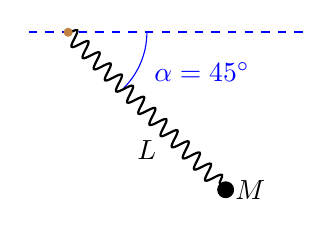
\begin{tikzpicture}[spring/.style={decorate,decoration={snake,amplitude=1mm,
      segment length=2mm},thick},>=latex]
  \draw[blue, dashed,thick] (0.5,4) -- (4,4);
  \draw[blue] (2,4) arc (0:-45:1);
  \draw[blue] (2.7,3.5) node {$\alpha = 45^\circ$};
  \draw[spring] (1,4) -- ++(2,-2) node [midway, below=7] {$L$};
  \filldraw[black] (3,2) circle (0.1) node[right] {$M$};
  \filldraw[brown] (1,4) circle (0.05);
\end{tikzpicture}
}

\taskpic{На гладком конусе с углом при вершине 120$^\circ$ шарнирно 
закреплен невесомый нерастяжимый стержень длиной $L$. К концу 
стержня прикреплен груз. Вся система вращается вокруг 
вертикальной оси. При какой частоте вращения груз разорвет 
стержень, если стержень выдерживает утроенный вес 
груза?}{
\begin{tikzpicture}[>=latex]
  \draw[very thick] ++(0.25,1) -- ++(30:2cm) --++(-30:2cm) -- cycle;
  \draw[thick,dashed] (2,3) -- ++(0,-2.5);
  \draw (2,2) -- ++(0,0.25) node (b) {} -- ++(210:1cm) node (a) {};
  \filldraw[brown] (b) circle (0.05);
  \shadedraw[shading=ball] (a) circle (0.2);
  \draw[blue] ($(a)+(0.4,0.6)$) node {$L$};
  \draw[thick,->] (2.3,3) arc (0:-180:0.3);
\end{tikzpicture}
}

\task{Сопротивление проволоки изменяется с температурой по закону 
$R = R_0(1 + \alpha t)$, где $R_0$ --- сопротивление при температуре, равной 
0$^\circ$C. Как должно изменяться подводимое к проволоке напряжение 
для того, чтобы температура проволоки линейно росла со временем? 
Теплоемкость проволоки равна $C$, отвода тепла нет.}

\taskpic{Заряженная частица $(q, m)$ может скользить без трения по 
проволочному кольцу радиусом $R$, расположенному вертикально. 
Какое вертикальное электрическое поле нужно приложить, чтобы 
частота малых колебаний частицы уменьшилась в два 
раза?}{
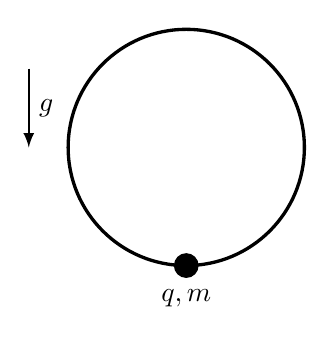
\begin{tikzpicture}[>=latex]
  \draw[very thick] (2.5,2) circle (1.5);
  \filldraw[black] (2.5,0.5) circle (0.15) node[below=5] {$q,m$};
  \draw[thick,->] (0.5,3) -- +(0,-1) node [midway,right] {$g$};
\end{tikzpicture}
}

\taskpic{В вертикальную трубу с бесконечными стенками поместили 
цилиндрическую капсулу. Сила трения между капсулой и стенками 
трубы прямо пропорциональна относительной скорости 
соприкасающихся поверхностей. Капсуле придали начальную 
линейную скорость, направленную вверх, и начальную угловую 
скорость. Когда капсула опустилась на начальную высоту, модуль 
линейной скорости изменился на $v$ относительно модуля начальной 
скорости, а угловая скорость стала равна $\omega$. При дальнейшем 
спуске капсула повернулась на угол $\alpha$ (на бесконечности). Время 
подъема от начальной высоты до наивысшей точки отличалось от 
времени спуска до начальной высоты на $T$. До какой максимальной 
высоты $H$ поднялась капсула, относительно начальной высоты, если 
радиус капсулы $R$, а ее масса распределена по боковой 
поверхности?}{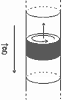
\includegraphics[width=1.5cm]{d11_18.png}}

\task{Электропоезд, составленный из одинаковых вагонов длиной $l$, 
начинает торможение в тот момент, когда первый вагон состава 
заходит в туннель длиной $L$. Двигаясь равнозамедленно, поезд 
останавливается в тот момент, когда его последний вагон выходит 
из туннеля. Известно, что пассажир первого вагона находился в 
туннеле в течение времени $T_1$, а последнего --- $T_N$. Чему равно 
количество вагонов в составе электропоезда?}

\taskpic{$N$ одинаковых небольших шариков подвешены к одной точке на 
невесомых нерастяжимых нитях длиной $L$. В начальный момент все 
маятники находятся в одной плоскости, содержащей вертикаль, 
проходящую через точку подвеса, и отклонены на углы $0 < \varphi_1 < 
\varphi_2 < \ldots < \varphi_n \ll \pi/2$. Начиная с первого, маятники 
последовательно отпускают без начальной скорости в моменты 
времени $\tau_1, \tau_2, \ldots, \tau_n$ соответственно. В какие моменты 
времени последний маятник будет находиться в точке своего 
начального положения? Все удары абсолютно 
упругие.}{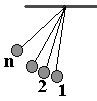
\includegraphics[width=3cm]{d11_20.png}}

\taskpic{Заряженной частице с массой $m$, помещенной в вакууме на 
границе двух областей, в которых созданы однородные магнитные 
поля $B_1$ и $B_2$ ($B_2 > B_1$), сообщают начальную скорость $v_0$, 
направленную перпендикулярно границе раздела. При каких 
значениях заряда частицы ее траектория пройдет через точку M, 
расположенную на расстоянии $L$ от точки 
старта?}{
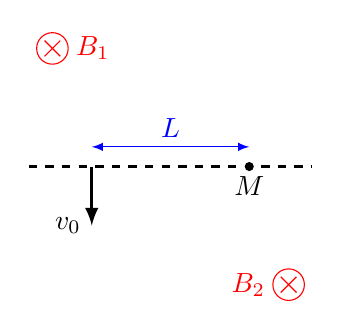
\begin{tikzpicture}[>=latex]
  \coordinate (a) at (3.5,0.5);
  \coordinate (b) at (0.5,3.5);
  \draw[red] (a) circle (0.2) node[left=5] {$B_2$};
  \draw[red] (a) ++ (-0.1,0.1) -- ++(0.2,-0.2);
  \draw[red] (a) ++ (0.1,0.1) -- ++(-0.2,-0.2);
  \draw[red] (b) circle (0.2) node[right=5] {$B_1$};
  \draw[red] (b) ++ (-0.1,0.1) -- ++(0.2,-0.2);
  \draw[red] (b) ++ (0.1,0.1) -- ++(-0.2,-0.2);
  
  \draw[dashed,thick] (0.2,2) -- ++(3.6,0);
  \draw[very thick,->] (1,2) -- ++(0,-0.75) node[left] {$v_0$};
  \filldraw[black] (3,2) circle (0.05) node[below] {$M$};
  \draw[blue,<->] (1,2.25) -- ++(2,0) node[fill=white,midway,above] {$L$};
\end{tikzpicture}
}

\taskpic{Найдите заряды на конденсаторах в схеме, изображенной на 
рисунке.}{
\begin{circuitikz}
  \draw[thick] (0,0) to[C, l_=$C_1$] (1.8,0) to [C, l_=$C_2$] (3.6,0) --
  ++(0,2.5) to [battery, l_=$\varepsilon_2$] (1.8,2.5);
  \draw[thick] (0,0) -- ++(0,2.5) to [battery,l^=$\varepsilon_1$] (1.8,2.5);
  \draw[thick] (1.8,0) to [C,*-*,l_=$C_3$] (1.8,2.5);
\end{circuitikz}
}

\task{С помощью кипятильника, рассчитанного на 110~В, можно 
вскипятить воду в чайнике за время $t$. Известно, что превышение 
мощности кипятильника на 20\% приводит к выходу его из строя. Как с 
помощью двух кипятильников на 110~В вскипятить такое же 
количество воды в чайнике, если напряжение в розетке 220~В? Какое 
время потребуется для этого? Потерями тепла пренебречь.}

\taskpic{По поверхности диэлектрической фигуры в форме телефонной 
трубки равномерно распределен заряд $Q > 0$. Фигура помещена в 
электрическое поле напряженностью $E$ так, что она может свободно 
вращаться вокруг точки A. В положении равновесия угол между 
отрезком AB и направлением электрического поля равен $\alpha$. Какую 
работу надо совершить, чтобы медленно повернуть фигуру в 
положение, когда отрезок AB направлен вдоль поля? Длина отрезка AB = 
$L$ , силой тяжести пренебречь.}{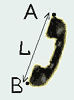
\includegraphics[width=2cm]{d11_24.png}}

\taskpic{Какую горизонтальную скорость необходимо сообщить очень 
маленькому мячику, лежащему на краю верхней ступеньки лестницы 
для того, чтобы первый отскок мяча произошел от ступеньки с 
номером $N$? Длины и высоты ступенек лестницы соответственно 
равны $b$ и $h$.}{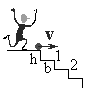
\includegraphics[width=2.5cm]{d11_25.png}}

\taskpic{Легкая нерастяжимая нить привязана в точке A к потолку, 
затем пропущена сквозь маленькую массивную бусинку, зацеплена 
за два блока B и C, и привязана к бусинке вторым концом. 
Первоначально бусинку удерживают так, что углы, которые нить 
образует с горизонталью, равны $\alpha$, $\beta$ и 90$^\circ$. Затем систему 
отпускают. Найдите вектор ускорения бусинки в начальный момент 
времени. Ускорение свободного падения $g$.}{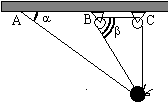
\includegraphics[width=3cm]{d11_26.png}}

\task{Тяжелый теплоизолированный контейнер массой $M = 10\mbox{ кг}$, 
содержащий $m = 1\mbox{ кг}$ газа, отпустили без начальной скорости с 
высоты $H = 15\mbox{ м}$. На какую высоту подскочит контейнер, если его 
соударение с землей абсолютно упругое? Сопротивлением воздуха 
пренебречь; считать, что колебания в газе быстро затухают.}

\taskpic{Зависимость тока от напряжения на элементе X приведена на 
графике. Постройте график зависимости тока от напряжения для 
схемы, изображенной на рисунке. Схема состоит из резисторов 
(номиналы указаны) и элементов 
X.}{
\begin{circuitikz}
  \draw[thick] (0.2,2) -- ++(0.3,0) -- ++(0,1) to [generic,l=$R$] (2,3) to
  [Do,l=$X$] (3.5,3) -- (3.5,2) -- (3.8,2);
  \draw[thick] (0.5,2) -- ++(0,-1) to [Do,l=$X$] (2,1) to [generic,l=$R$]
  (3.5,1) -- ++(0,1);     
\end{circuitikz}
}
\begin{figure}[h]
  \centering
  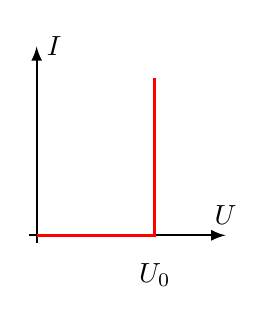
\begin{tikzpicture}[>=latex]
    \draw[thick,->] (0.4,0.5) -- ++(2.5,0) node[above] {$U$};
    \draw[thick,->] (0.5,0.4) -- ++(0,2.5) node[right] {$I$};
    \draw[red,very thick] (0.5,0.5) -- ++(1.5,0) -- ++(0,2);
    \draw (2,0) node {$U_0$};
  \end{tikzpicture}
\end{figure}

\task{Вертикально в землю вкопан длинный стержень, по которому 
могут без трения двигаться две маленькие бусинки. Бусинки упруго 
соударяются друг с другом, а нижняя упруго соударяется с землей. 
Верхняя, которая в $n = 10^4$ раз тяжелее нижней, практически 
неподвижно зависла на высоте $H = 1\mbox{ м}$ над Землей. Определите 
скорость нижней бусинки.}

\taskpic{Тележка массой $M$, двигающаяся со скоростью $V$ прямолинейно, 
наталкивается на легкую пружину длиной $L$, прикрепленную к стене. 
На тележке закреплен хрупкий предмет массы $m$, который 
разбивается, если его перемещать с ускорением больше чем $a_0$. 
Какой должна быть жесткость пружины, чтобы в процессе 
столкновения хрупкий предмет не разбился? Трением тележки о пол 
пренебречь. Пружину считать идеальной при любой длине от 0 до 
$L$.}{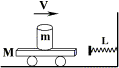
\includegraphics[width=3cm]{d11_30.png}}

\taskpic{К сосуду подключен нагреватель постоянной мощности, и в 
него налито некоторое количество жидкости. Дан график 
зависимости температуры жидкости от времени. Жидкость в сосуде 
хорошо перемешивается, поэтому можно считать температуру 
одинаковой по всему объему. Опыт повторяют с теми же начальными 
условиями, однако теперь в момент времени $t_1 = 5\mbox{ мин}$ массу 
жидкости увеличивают вдвое, не меняя ее температуру. Найдите при 
этом температуру жидкости в момент времени $t_2 = 10\mbox{ мин}$. 
Считайте, что мощность тепловых потерь не зависит от объема 
жидкости.}{
\begin{tikzpicture}[>=latex,domain=0:3]
  \draw[help lines,xstep=0.75,ystep=0.5] (0,0) grid (3.1,2.8);
  \draw[->] (0,0) --++(3.2,0);
  \draw (1.5,-0.7) node {\tiny{$t$, мин}};
  \draw[->] (0,0) --++(0,3) node[right] {\tiny{$T, ^\circ$C}};
  \draw[red,thick] plot(\x,{2-exp(-1.5*\x)});
  \foreach \x in {2.5,5,7.5,10}
  \draw (\x*3/10,0.05) -- ++(0,-0.1) node[anchor=north] {\tiny{$\x$}};
  \foreach \y in {0,20,40,60,80,100}
  \draw (0.05,\y/40) -- ++(-0.1,0) node[anchor=east] {\tiny{$\y$}};
\end{tikzpicture}
}

\task{Воздушный шарик представляет собой тонкую резиновую 
оболочку, имеющую в нерастянутом состоянии радиус $r_0$ и толщину 
$d_0$. Материал шарика обладает модулем Юнга $E$ и при растяжении 
подчиняется следующему закону: произведение относительного 
удлинения на модуль Юнга равно механическому напряжению. Кроме 
того, при растяжении объем материала не изменяется. Шарик 
помещают в вакуум и начинают надувать газом с молярной массой $\mu$ 
и температурой $T$. Определите зависимость радиуса шарика и 
давления в нем от массы $m$ закачанного газа. Постройте графики 
этих зависимостей. (Напоминаем, что механическое напряжение $\sigma$ 
равно отношению растягивающей силы к площади поперечного 
сечения образца).}

\taskpic{С гладкого цилиндра радиуса $R$ соскальзывает тонкая 
однородная веревка длины $\pi R/2$, лежащая в вертикальной 
плоскости. Найдите силу натяжения веревки в точке A ($0 < \alpha < \pi/2$). 
Масса веревки $m$, ускорение свободного падения 
$g$.}{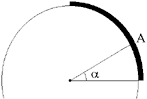
\includegraphics[width=3cm]{d11_33.png}}

\taskpic{В длинном цилиндрическом сосуде находится $\nu = 1\mbox{
моль}$ гелия, заключенный между теплоизолированными боковой стенкой и
поршнем, соединенных друг с другом резинкой с нулевой начальной
длинной. Коэффициент жесткости резинки равен $k = 3{,}46\mbox{
Н/м}$. Весь цилиндр помещен в очень горячую однородную среду. Поршень
удерживают на расстоянии $l = 1\mbox{ м}$ от левого торца, при этом
температура газа возрастает на $t = 1\mbox{ К}$ за каждые $\tau =
20\mbox{ с}$.  Поршень отпускают; в начальный момент силы, действующие
на поршень, скомпенсированы. Постройте график зависимости длины
резинки $L$ от времени. Трения между поршнем и цилиндром нет. $R =
8{,}31\mbox{ Дж/(моль}\cdot\mbox{К)}$.}{
\begin{tikzpicture}[>=latex,domain=0:3]
  \draw[pattern=north east lines] (3.8,2.5) --++(0,0.5) --++(-3.8,0)
  -- ++(0,-2) -- ++(3.8,0) -- ++(0,0.5) -- ++(-3.3,0) --++(0,1)
  --++(3.3,0) -- cycle;
  \draw (3.8,2.5) -- (0.5,2.5) -- (0.5,1.5) -- (3.8,1.5);
  \filldraw[gray] (0.5,2.5) rectangle ++(0.2,-1);
  \draw[pattern=dots,pattern color=green] (0.7,2.5) rectangle
  ++(2,-1);
  \draw[very thick] (0.7,2) -- ++(2,0);
  \filldraw[black] (2.7,2.5) rectangle ++(0.2,-1);
  \draw[blue,thick,->] (2,3.5) node[right] {$L$} to[out=180,in=90] (1.5,2.1);
\end{tikzpicture}
}

\taskpic{Однородный шар массой $M$, равномерно заряженный по объему 
электрическим зарядом $Q$, закреплен на невесомом нерастяжимом 
канате и вращается в плоскости, перпендикулярной линиям 
магнитного поля $B$ с постоянной угловой скоростью $\omega$. Известно, 
что при увеличении длины каната в $n$ = 3~раза сила его натяжения 
увеличивается в $k$ = 2~раза. Чему равна величина вектора магнитной 
индукции, если известно, что после выключения магнитного поля 
сила натяжения нити стала такой же, как до увеличения длины нити? 
Сила тяжести отсутствует.}{
\begin{tikzpicture}[>=latex]
  \draw[dashed,blue] (2,2) circle (1.5);
  \draw[fill=brown] (2,2) circle (0.05);
  \draw[very thick] (2,2) -- ++(225:1.5);
  \shadedraw[shading=ball] ($(2,2)+(225:1.5)$) circle (0.2) node[right=5]
  {$M,Q$};
  \draw[red] (3,3.5) circle (0.15) node[right] {$B$};
  \draw[red] ($(3,3.5) +(0.05,0.05)$) -- ++(-0.1,-0.1);
  \draw[red] ($(3,3.5) +(-0.05,0.05)$) -- ++(0.1,-0.1);
\end{tikzpicture}
}

\task{Тонкая массивная шайба надета на длинный стержень радиуса $R$. 
Когда шайбу закрутили вокруг стержня с угловой скоростью $\omega$, 
оказалось, что она останавливается через время $t_0$. В другой раз 
шайбу закрутили с той же угловой скоростью и одновременно 
придали ей скорость $v_0$ вдоль стержня. Какой путь пройдет по 
стержню шайба до остановки? Зазора между шайбой и стержнем нет.}
